\chapter{Implementation}

\section{Software}

\subsection{OpenVPN}
% By default, point-to-point, but since the version 2.0 can be configured in server mode, hence being able to manage hundreds of clients.

% Pages 20-21, I have the workflow of openvpn, showing the encryption happening before the fragmentation.
\lstset{language=c}
\lstset{commentstyle=\color{colComments}\textit,
float=hbp,%
basicstyle=\ttfamily\footnotesize, %
identifierstyle=\color{colIdentifier}, %
keywordstyle=\color{colKeys}, %
stringstyle=\color{colString}, %
columns=flexible, %
tabsize=2, %
extendedchars=true, %
showspaces=false, %
showstringspaces=false, %
numbers=left, %
numberstyle=\tiny, %
breaklines=true, %
breakautoindent=true, %
captionpos=b}
\begin{lstlisting}[caption=openvpn compress then encrypt -- sample from \texttt{forward.c}, label=list:]
/* Compress, fragment, encrypt and HMAC-sign an outgoing packet. */
void encrypt_sign (struct context *c, bool comp_frag)
{
	struct context_buffers *b = c->c2.buffers;
	const uint8_t *orig_buf = c->c2.buf.data;

	if (comp_frag){
	/* Compress the packet. */
		if (lzo_defined (&c->c2.lzo_compwork))
			lzo_compress (&c->c2.buf, b->lzo_compress_buf, &c->c2.lzo_compwork, &c->c2.frame);
	/* Fragment the packet. */
		if (c->c2.fragment)
			fragment_outgoing (c->c2.fragment, &c->c2.buf, &c->c2.frame_fragment);
	}

  /* Encrypt the packet and write an optional HMAC signature. */
	openvpn_encrypt (&c->c2.buf, b->encrypt_buf, &c->c2.crypto_options, &c->c2.frame);
}
\end{lstlisting}

\begin{figure}[ht]
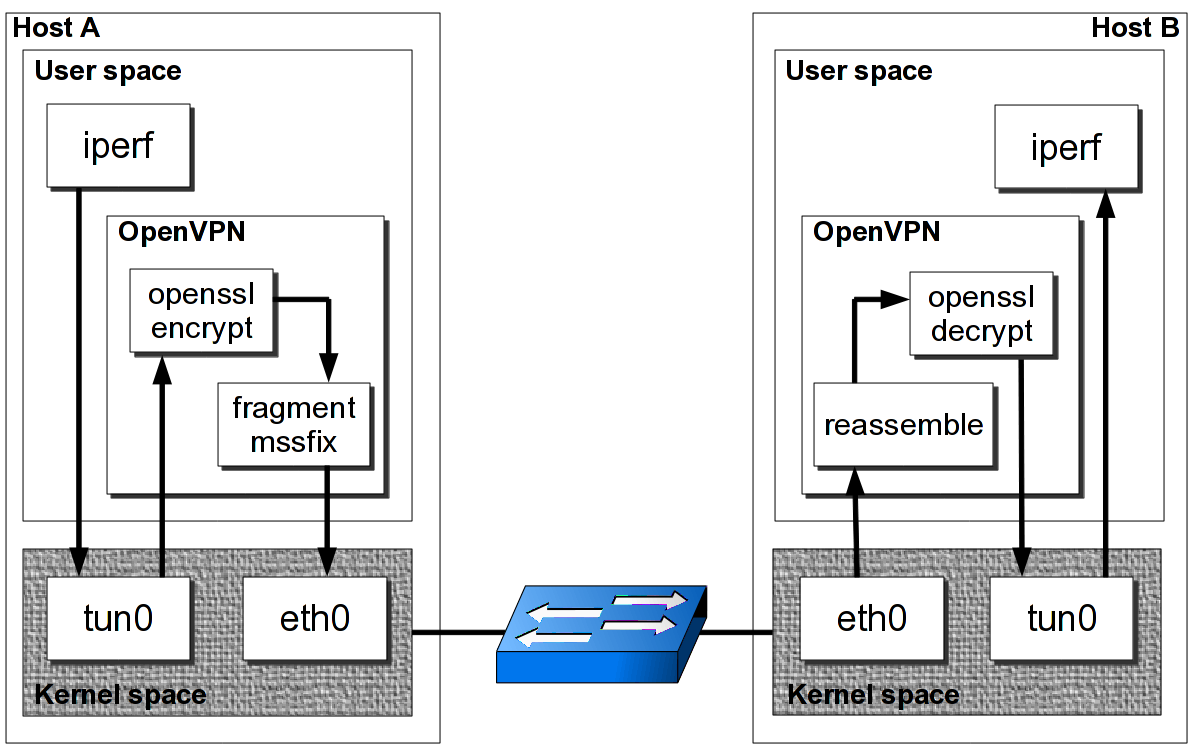
\includegraphics[width=\textwidth]{OpenVPN-packetflow}
\caption{OpenVPN packet flow as advertized on the openVPN wiki.}
\label{fig:openvpn-packet-flow}
\end{figure}

\subsection{OpenSSL}
% Talk about the debug flags in the compilation and show it has close to none impact on the performance (using openssl speed. openssl speed is a relevant test because openssl uses 100% of the CPU, hence maximizing the potential performance reduction.)

% Talk about the assembly implementation, maybe show the difference in an appendice with the C implementation. Not /that/ interresting.

\subsection{OpenSSH}
% Talk about the MAC=none patch
% connection using SSL/TLS, then AES, but without fragmentation (unlike openvpn)


\subsection{Strongswan}


\subsection{Linux drivers}
% Mention the fact that we use the assembly implementation of AES, not the generic C one.

\section{Offload}

\subsection{Silex engine}

\subsection{BA411E Driver}

\subsection{BA414E Driver}